\chapter{Các công trình liên quan}

% Hiện nay, số lượng các đối tượng vật thể tồn tại trong cuộc sống là rất nhiều và vô cùng đa dạng. Mỗi loại vật thể lại có đặc điểm riêng về hình dạng, kích thước, đặc trưng riêng. Hơn thế nữa, trong cùng một loại đối tượng thì mỗi vật thể cũng có nhiều biến thể, dẫn tới sự khó khăn rất lớn trong việc xác định một mô hình, kích cỡ cố định của mỗi loại vật thể. \\
Sau đây, nhóm sẽ trình bày những tìm hiểu và nghiên cứu của nhóm về quá trình hình thành và phát triển của các phương pháp dự đoán độ sâu cũng như phát hiện và phân mảnh vật thể mà các nhóm nghiên cứu trong nước và trên thế giới đã thực hiện.

%Với mục tiêu của nhóm là có thể ước lượng được khoảng cách của vật thể từ một ảnh RGB, nhiệm vụ đầu tiên cần phải thực hiện đó chính là biết đối tượng vật thể nằm ở đâu, vị trí nào trong bức ảnh. Do vậy, nhóm quyết định áp dụng các kết quả đã đạt được hiện có về phát hiện, bao đóng, phân mảnh vật thể để có thể cải thiện độ chính xác của việc ước lượng khoảng cách. Dưới đây, nhóm xin trình bày quá trình tìm hiểu, cũng như áp dụng các phương thức để thực hiện phát hiện, bao đóng và phân mảnh vật thể.

\section{Dự đoán độ sâu}
Nhóm đã thực hiện những khảo sát trong nước nhưng nhóm chưa tìm được các công trình có liên quan trong khoảng thời gian cho phép, cho nên những nghiên cứu và công trình dưới đây mà nhóm trình bày thuộc các công trình của các nhóm nghiên cứu quốc tế.\\

Bài toán dự đoán độ sâu từ ảnh nguyên gốc dựa trên stereo vision \cite{sinz2004learning,memisevic2011stereopsis} sử dụng những cặp ảnh của cùng một khung cảnh để tái tạo lại hình dạng trong không gian thực. Nhưng sau đó bài toán được tiếp cận theo các hướng chính như sau:
\subsubsection{Dự đoán độ sâu dựa vào ảnh RGB}
Những phương pháp cổ điển để dự đoán độ sâu từ ảnh RGB chủ yếu dựa trên các đặc trưng được lấy từ bức ảnh một cách thủ công, sử dụng mô hình đồ thị xác suất (problistic graphical model) đưa ra những giả định về hình học của khung cảnh để giải quyết vấn đề \cite{hoiem2005geometric,liu2010single, saxena2006learning, saxena2009make3d}, một trong những công trình đầu tiên bởi Saxena et al. \cite{saxena2006learning}, sử dụng mô hình Markov Random Field (MRF) để suy diễn độ sâu từ những đặc trưng cục bộ cho đến đặc trưng toàn cục được trích xuất từ ảnh. Sau đó họ đã tiến hành mở rộng công trình của mình để tái tạo lại khung cảnh 3 chiều \cite{saxena2009make3d}(3D scene reconstruction). Từ đề tài này, Liu et al. \cite{liu2010single} kết hợp bài toán phân đoạn ngữ nghĩa (semantic segmentation) với bài toán ước lượng độ sâu, tại đó nhãn dự đoán được sử dụng như là ràng buộc thêm để quá trình tối ưu trở nên dễ dàng hơn. Những hướng tiếp cận không tham số (non-parametric) \cite{karsch2014depth, liu2011sift, liu2014discrete, konrad20122d}, với hướng đi này ta sẽ thường so trùng đặc trưng (GIST, HOG) giữa ảnh RGB mà ta muốn có ảnh độ sâu với những ảnh của cơ sở dữ liệu RGB-D, nhằm tìm ra những ảnh tương tự với nó nhất, sau đó dùng ảnh độ sâu của những ảnh này tiến hành sinh ra ảnh độ sâu cuối cùng cho ảnh RGB. Cần chú ý rằng những phương pháp này dựa trên giả định rằng những khung cảnh tương tự nhau thì có phân bố độ sâu cũng tương tự nhau.\\

Gần đây, nhờ những bước tiến lớn của học sâu mà nó đã dẫn dắt hướng nghiên cứu sang sử dụng CNN để ước lượng độ sâu. Bởi vì bài toán này khá tương đồng với bài toán gán nhãn ngữ nghĩa (semantic labeling), nên hầu hết các nghiên cứu đã xây dựng mạng CNN của họ dựa trên những kiến trúc đã chiến thắng trong cuộc thi ImageNet Large Scale Visual Recognition Challenge (ILSVRC) \cite{Imagenet}. Eigen et al. \cite{Eigen2014} là nhóm tiên phong sử dụng CNN để dự đoán độ sâu từ một ảnh đơn, kiến trúc của nhóm này gồm 2 phần chồng lên nhau. Phần đầu gọi là coarse-scale network dựa trên AlexNet \cite{Krizhevsky2012}, nó sẽ dự đoán độ sâu của bức ảnh ở mức toàn cục, sau đó kết quả này được tinh chỉnh ở mức cục bộ bởi fine-scale network. Họ còn tiến hành mở rộng công trình của mình để có thể dự đoán thêm được bề mặt và nhãn (predict surface normal and semantic labeling) với một mô hình sâu hơn dựa trên VGG \cite{Simonyan2014} đó là một kiến trúc 3 thành phần để giải quyết được cả 3 bài toán chỉ từ một bức ảnh đơn \cite{Eigen2015}. Laina et al. \cite{laina2016deeper} và Cao et al. \cite{cao2017estimating} dựa trên Residual Nerual Network (ResNet) \cite{KHe2015} nó đã đứng hạng nhất ở bài toán phân loại và nhận diện của ILSVRC và COCO 2015. Cụ thể Laina et al. \cite{laina2016deeper} đã hồi quy giá trị độ sâu bằng một mạng có kiến trúc bao gồm 2 phần, phần đầu dựa trên ResNet, phần sau nhóm của Laina đã đề xuất các khối Up-convolution và Up-projection để sinh ra ảnh độ sâu có độ phân giải cao. Thay vì hồi quy, Cao et al. \cite{cao2017estimating} đã định hướng bài toán ước lượng độ sâu thành bài toán phân loại có nghĩa là thay vì dự đoán chính xác giá trị độ sâu tại mỗi điểm ảnh thì nhóm của Cao sẽ phân loại xem điểm ảnh có giá trị độ sâu thuộc khoảng nào, kiến trúc mà nhóm của Cao đề xuất cũng gồm 2 phần, phần đầu là mạng CNN dựa trên ResNet để phân loại, kết quả này sau đó được tinh chỉnh bằng cách áp dụng fully connected conditional random field được đề xuất bởi \cite{krahenbuhl2011efficient}.

\subsubsection{Kết hợp cảm biến (sensor fusion)}
Nhằm cải thiện chất lượng của ảnh độ sâu được dự đoán thì ngoài sử dụng ảnh RGB, nhiều nhóm nghiên cứu đã sử dụng thêm thông tin được lấy từ các cảm biến khác. Cụ thể  Macini et al.  \cite{mancini2016fast} đã đề xuất một mạng CNN nhận ảnh RGB và ảnh optical flow tương ứng làm đầu vào để dự đoán khoảng cách. Liao et al. \cite{liao2017parse} thì sử dụng máy quét laze (2D laser scanner) dùng để tạo ra tín hiệu độ sâu (additional reference depth signal) như là đầu vào và đạt được độ chính xác cao hơn khi chỉ sử dụng một mình ảnh RGB. Đặc biệt Ma et al. \cite{Ma2017SparseToDense} đã xem xét sử dụng ảnh độ sâu thưa kết hợp với ảnh RGB để sinh ra ảnh độ sâu dày dựa trên kiến trúc của Laina \cite{laina2016deeper} và kết quả cho thấy khá ấn tượng.\\

Kết thúc phần khảo sát các công trình thực hiện dự đoán độ sâu. Nhóm đã chọn đi theo hướng tiếp cận của Ma \cite{Ma2017SparseToDense} cho phần ước lượng độ sâu của nhóm, chi tiết sẽ được trình bày rõ ở chương 4.



\section{R-CNN} 

\subsection{Mô tả chung}

R-CNN \cite{Girshick2013} thực hiện việc tính toán theo các tầng khác nhau được thể hiện ở hình \ref{fig:rcnn}. Đầu tiên, sẽ khởi tạo các vùng mà sẽ được quan tâm (the regions of interest, RoIs). RoIs chính là các bao đóng các vùng độc lập mà trong nó có thể chứa đối tượng. R-CNN sử dụng Selective Search để tạo ra các RoIs.\\

Tiếp theo, một mạng CNN sẽ được dùng để trích xuất các đặc điểm từng mỗi vùng được đề xuất. Vùng này được co giãn theo tỉ lệ để phù hợp với kích thước input của CNN và được đưa vào mạng. Sau khi mạng CNN trích xuất các đặc điểm từ input, thì những đặc điểm này sẽ được đưa vào SVM để thực hiện việc phân loại.

\begin{center}
   \begin{figure}[H]
   \begin{center}
     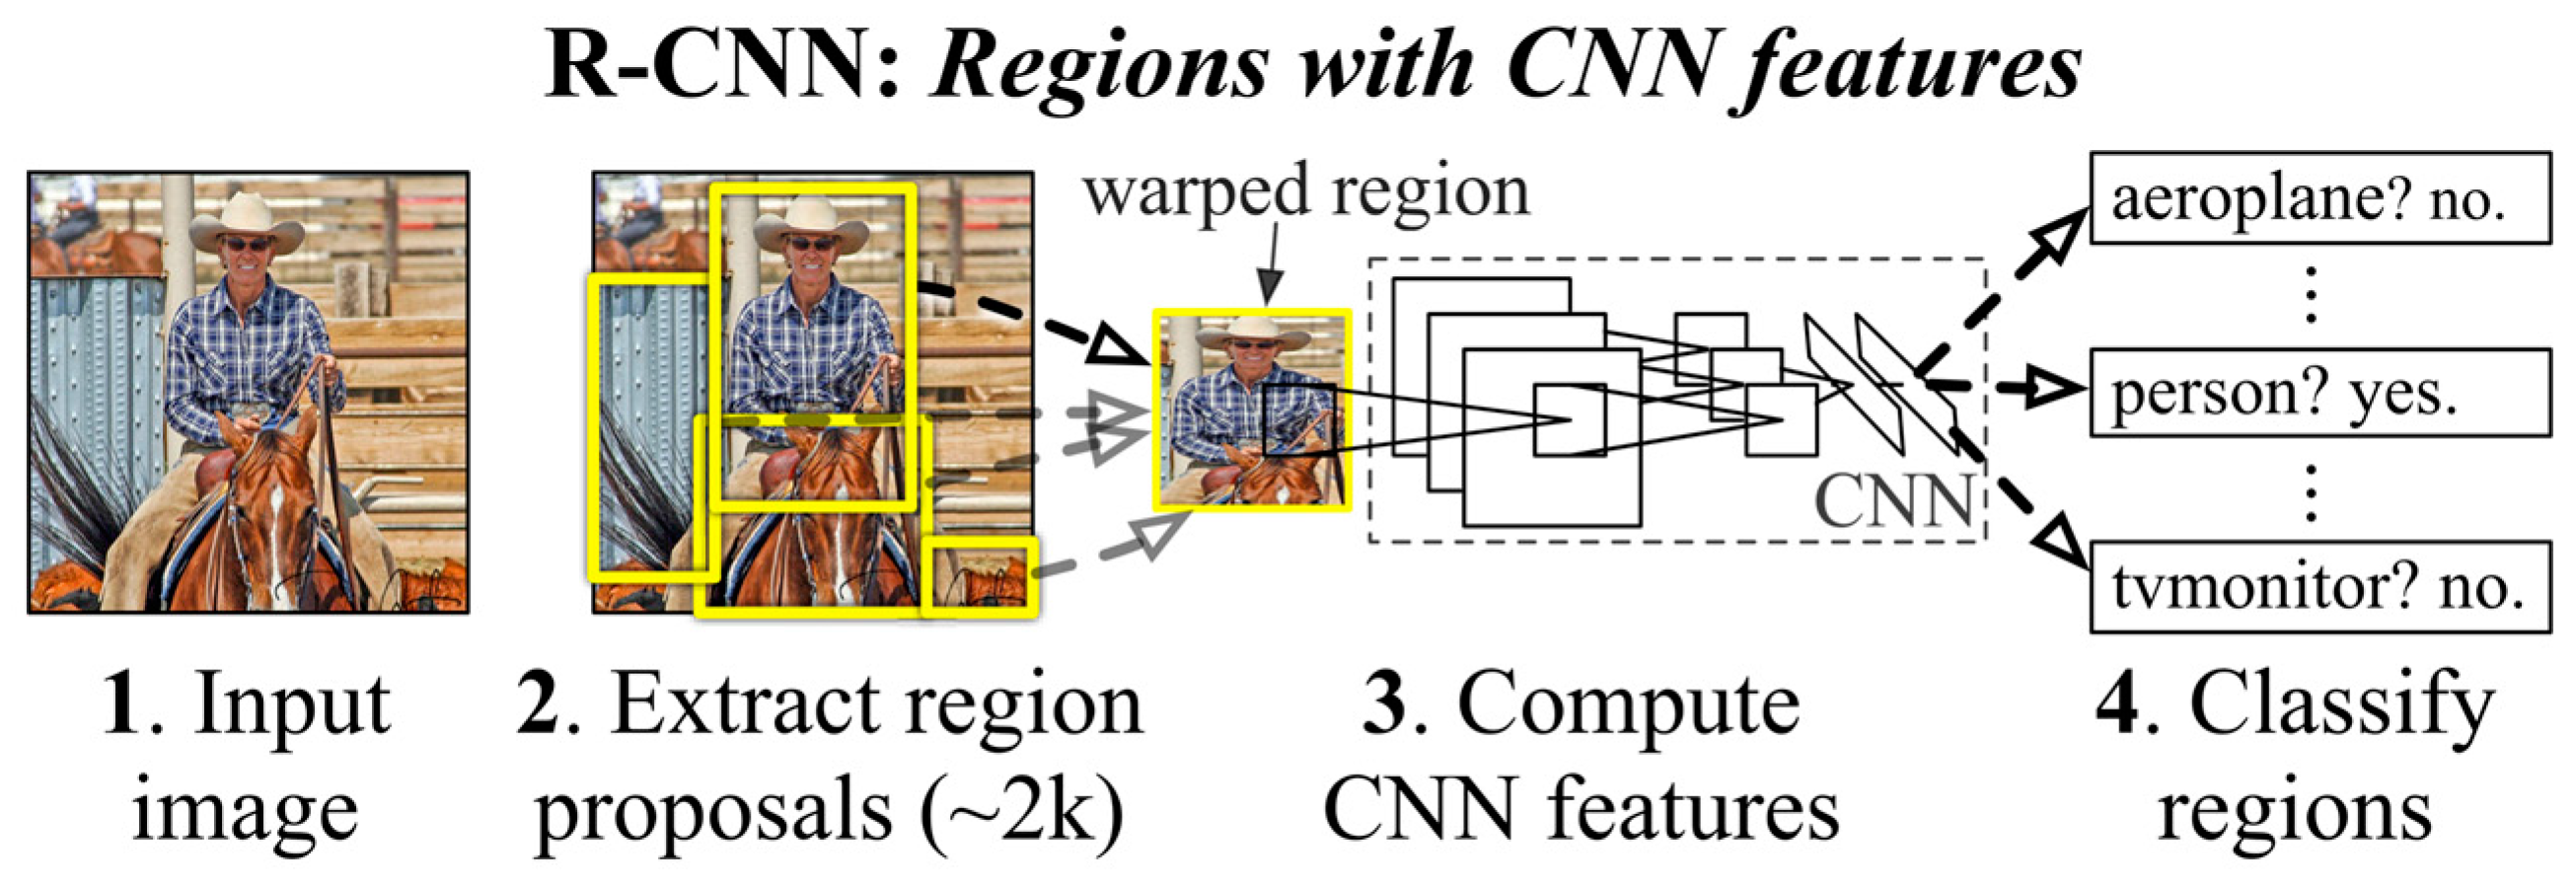
\includegraphics[scale=1.3]{image/rcnn}
    \end{center}
    \caption{Stages of R-CNN}
    \label{fig:rcnn}
    \end{figure}
\end{center}

%Phương thức này được huấn luyện ở nhiều tầng, đầu tiên, mạng %CNN sẽ được huấn luyện. Tiếp theo, SVM sẽ được điều chỉnh dựa %vào các đặc điểm được trích xuất từ mạng CNN. Cuối cùng, %phương thức khởi tạo các vùng được quan tâm được huấn luyện.

\subsection{Hạn chế của R-CNN}

R-CNN là một phương thức nền tảng quan trọng trong phát hiện vật thể, bởi vì nó cung cấp giải pháp đầu tiên cho việc sử dụng CNN cho phát hiện vật thể. Và bởi vì là tiên phong, nên nó có những hạn chế và càng ngày được cải thiện về sau.\\

Những vấn đề chính của R-CNN:
\begin{enumerate}
	\item Quá trình huấn luyện gồm nhiều bước, được mô tả như ở trên.
	\item Với cả việc huấn luyện SVM và phương thức khởi tạo vùng quan tâm, toàn bộ dữ liệu được lưu giữ trên đĩa. Điều này yêu cầu nhiều ngày tính toán cũng như không gian lưu trữ rất lớn.
	\item Cuối cùng, và cũng là quan trọng nhất, việc phát hiện vật thể được thực hiện khá chậm, yêu cầu khoảng một phút cho mỗi ảnh, thậm chí là trên GPU. Bởi vì việc tính toán trên CNN được thực hiện độc lập giữa mỗi vùng được đề xuất,  kể cả những vùng từ cùng một ảnh, có trùng với các vùng khác.
\end{enumerate}

\section{Fast R-CNN} 

Ngay từ cái tên, Fast R-CNN \cite{Girshick2015FastR} đã thể hiện việc nó hình thành dựa trên ý tưởng chính của R-CNN. Nhưng thay vì đưa vào CNN những vùng được đề xuất riêng biệt, thì Fast R-CNN đưa vào mạng CNN toàn bộ bức ảnh để trích xuất đặc điểm.

\subsection{Mô tả chung}

\begin{center}
   \begin{figure}[H]
   \begin{center}
     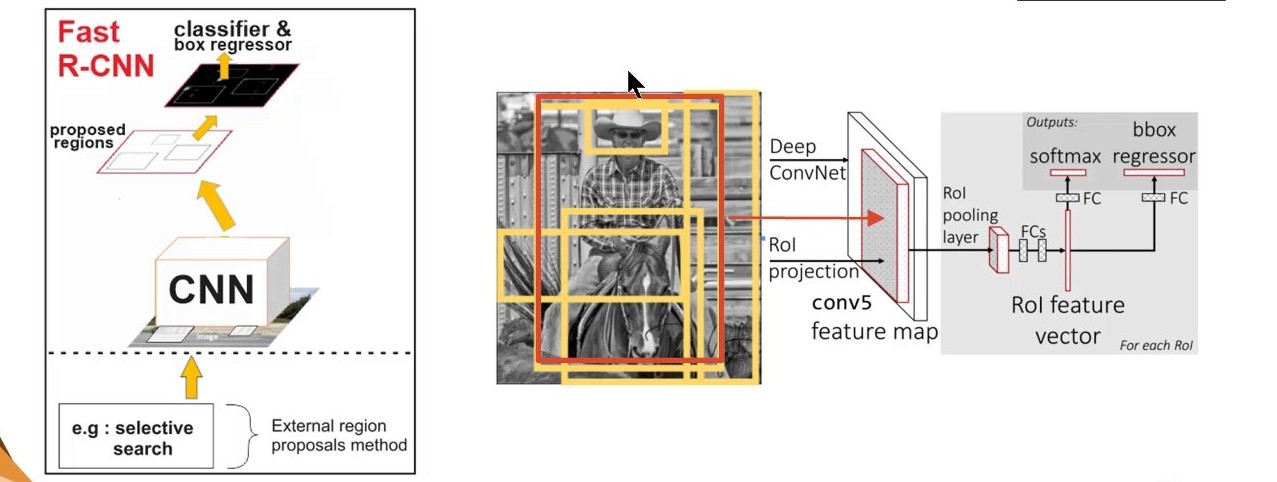
\includegraphics[scale=0.3]{image/fast_rcnn_1}
    \end{center}
    \caption{Stages of Fast R-CNN}
    \label{ref_fast-rcnn}
    \end{figure}
\end{center}

Kiến trúc chung của Fast R-CNN được thể hiện như trên hình 4.1. Fast R-CNN nhận input là bức ảnh và vùng được quan tâm tính toán từ hình ảnh (Region of Interests,RoIs). Cũng giống như R-CNN, thì các RoIs cũng được khởi tạo từ Selective Search, nhưng không phải được thực hiện trên ảnh gốc mà được thực hiện trên feature maps được tạo ra thông qua các lớp convolutional và lớp max-pooling.\\

Khối đặc điểm được trích xuất từ bức ảnh (feature map) kết hợp với các RoIs sẽ là input của lớp RoI pooling. Lớp này có nhiệm vụ tạo ra output có kích cỡ đồng nhất cho mỗi vùng được đề xuất từ feature map. Các vector output từ lớp RoI-pooling sẽ là input của một lớp fully-connected được kết nối với 2 lớp: một lớp softmax để tạo ra xác suất ước tính cho việc phân loại  đối tượng và một lớp bounding-box regressor để ước tính bao đóng cho đối tượng.\\

\subsection{Nhận xét}

Toàn mạng có thể được huấn luyện sử dụng \textit{backpropagation} và \textit{stochastic gradient descent}. Các RoI sẽ được gán nhãn lớp nếu nó giao với bao đóng thật của đối tượng hơn 0.5, ngược lại, những RoI khác sẽ thuộc về lớp nền. Trong việc phân lớp, RoIs từ cùng một ảnh sẽ chia sẻ tính toán và sử dụng bộ nhớ. Theo như kết quả hiện thực, thì Fast R-CNN đã đạt được thời gian ngắn hơn rất nhiều trong trong huấn luyện và test so với R-CNN, cũng như đạt được kết quả tốt hơn trong việc phát hiện vật thể.

\section{Faster R-CNN}

\subsection{Mô tả chung}

Faster R-CNN \cite{Ren2015} là phương pháp nhóm đang nghiên cứu để thực hiện phát hiện vật thể trong không gian 2 chiều. Cũng giống như Fast R-CNN dựa trên nền tảng của R-CNN để đưa ra những cải tiến, thì Faster R-CNN cũng dựa trên Fast R-CNN để đưa ra những thay đổi, hướng tới việc phát hiện vật thể theo thời gian thực. \\

\begin{center}
   \begin{figure}[H]
   \begin{center}
     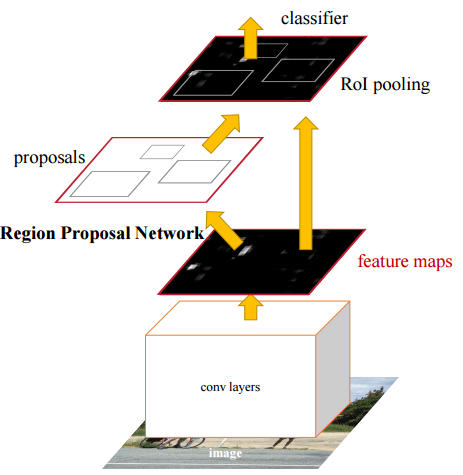
\includegraphics[scale=0.6]{image/faster_rcnn_1}
    \end{center}
    \caption{Faster R-CNN}
    \label{faster_rcnn}
    \end{figure}
\end{center}

Ý tưởng chính của Faster R-CNN là dùng chung các lớp convolutional cho việc khởi tạo các vùng đề xuất và cho việc phát hiện vật thể, ở đây, chính là các feature maps. Sự khác biệt chính giữa Fast R-CNN và Faster R-CNN chính là trong việc khởi tạo các vùng được đề xuất. Với R-CNN và Fast R-CNN, việc khởi tạo các vùng được đề xuất đều sử dụng Selective Search. Với Faster R-CNN, thay vì sử dụng Selective Search, Region Proposal Network được áp dụng và cho thấy được kết quả tốt hơn, không chỉ về chi phí tính toán mà cũng như thời gian thực thi. \\

Mạng CNN sẽ nhận một ảnh vào như là input. Feature maps sẽ được tạo ra từ mạng CNN, và nó được đưa vào như là input của RPN (region proposal network). Output của RPN kết hợp với feature maps sẽ tiếp tục là input của lớp phân loại cuối cùng, lớp này hình thành theo cấu trúc của Fast R-CNN. \\

Do sự chia sẻ kết quả feature map từ các lớp convolutional cho  việc khởi tạo các vùng được đề xuất, nên thời gian tính toán cũng như hiệu quả tính toán được cải thiện khá nhiều.

\subsection{Region Proposal Networks}
Như đã được đề cập nhiều ở trên, RPN nhận một ảnh là input và output chính là một tập các vùng được đề xuất có thể chứa đối tượng.Với convolutional feature map chúng ta có được sau khi đưa ảnh qua mạng convolutional ban đầu, sử dụng cửa sổ trượt với kích cỡ nxn trên feature map nhận được.\\

\begin{center}
   \begin{figure}[H]
   \begin{center}
     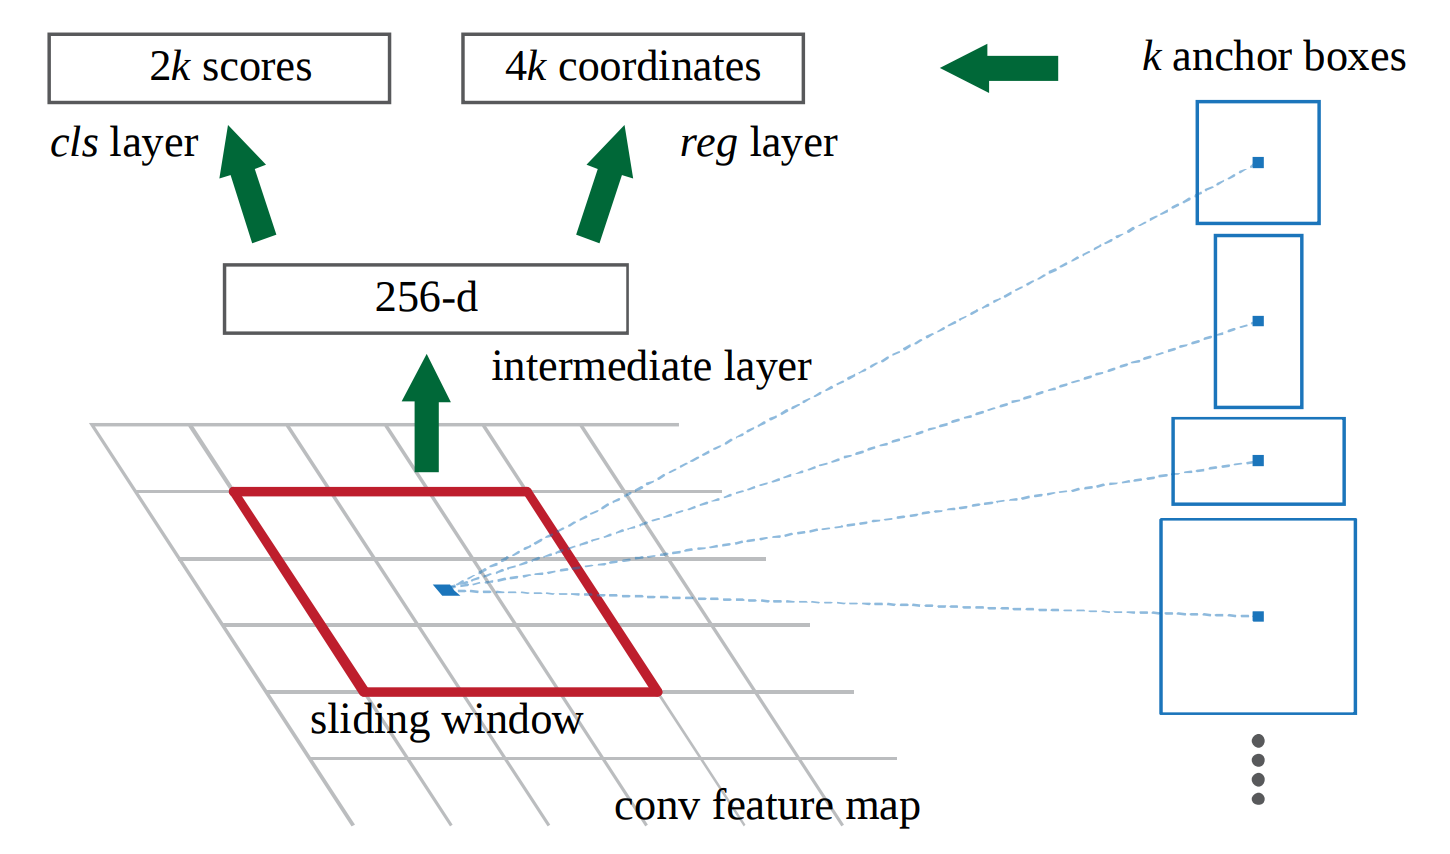
\includegraphics[scale=0.25]{image/anchor}
    \end{center}
    \caption{Region Proposal Network}
    \label{RPN}
    \end{figure}
\end{center}
Tại mỗi vị trí của cửa sổ trượt, Faster R-CNN đưa ra nhiều vùng đề xuất, và  số  những vùng với xác suất cao nhất có thể chứa vật thể tại mỗi vị trí là k. Do vậy, với lớp \textit{reg} sẽ có 4k output đại diện cho vị trí của vùng được đề xuất đó, và lớp \textit{cls} sẽ có output là 2k điểm ước tính xác suất có hoặc không có vật thể trong mỗi vùng đề xuất. Mỗi vùng trong k vùng được đề xuất ở trên được gọi là anchor. Mỗi anchor được đặt tại chính giữa ở mỗi của sổ trượt, và được phối hợp với tỉ lệ thu phóng (scale), và tỉ lệ cạnh (aspect ratio) nhất định. Mặc định, Faster R-CNN sử dụng 3 tỉ lệ thu phóng và 3 tỉ lệ cạnh, do đó k=9 anchors tại mỗi cửa sổ trượt.

% \begin{center}
%    \begin{figure}[htp]
%    \begin{center}
%      \includegraphics[scale=0.5]{image/anchor_1}
%     \end{center}
%     \caption{Anchor}
%     \label{ref_sigmoid}
%     \end{figure}
% \end{center}

\subsection{Nhận xét}

\begin{center}
   \begin{figure}[H]
   \begin{center}
     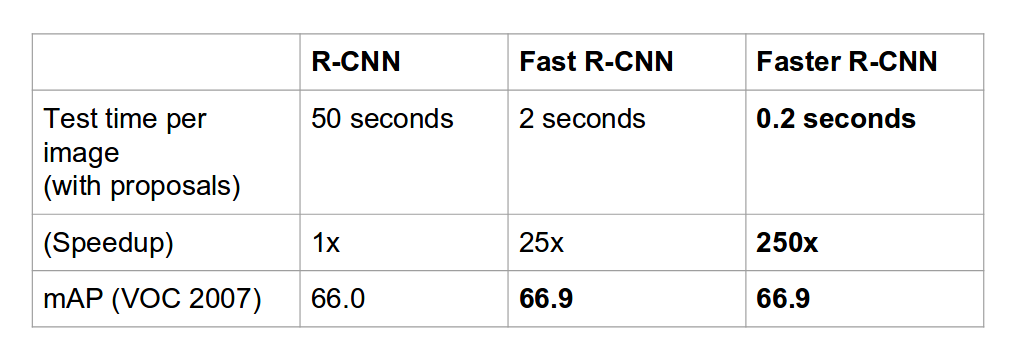
\includegraphics[scale=0.4]{image/fasterrcnn_result}
    \end{center}
    \caption{Faster R-CNN result}
    \label{ref_fasterrcnn_result}
    \end{figure}
\end{center}

Faster R-CNN cho thấy sự hiệu quả trong việc phát hiện vật thể khi thực hiện trong thời gian 200ms/1 ảnh, nhỏ hơn rất nhiều Fast R-CNN với thời gian 2s/1 ảnh. Faster R-CNN đã hướng đến phát hiện vật thể trong thời gian thực, phục vụ những nhu cầu hiện nay.\\

Ngoài ra, không chỉ Faster R-CNN, cũng có rất nhiều phương thức thực hiện việc phát hiện vật thể hiệu quả, nhanh chóng như SSD, YOLO ...\\


\section{Mask RCNN}

Dựa trên cấu trúc Faster RCNN, Mask RCNN \cite{He2017MaskR} ra đời đã cho kết quả rất tốt trong nhiệm vụ phân đoạn vật thể. Mask RCNN đã sử dụng ResNet, Feature Pyramid Network (FPN) nhằm trích xuất đặc điểm từ ảnh, đây là một trong những yếu tố quan trọng giúp Mask RCNN đạt được kết quả cao cả về tốc độ, lẫn độ chính xác. Với việc kết hợp sử dụng ResNet và FPN, thì mô hình đã có những feature maps rất tốt, để thực hiện bao đóng và segmengation vật thể. \\


\begin{center}
   \begin{figure}[H]
   \begin{center}
     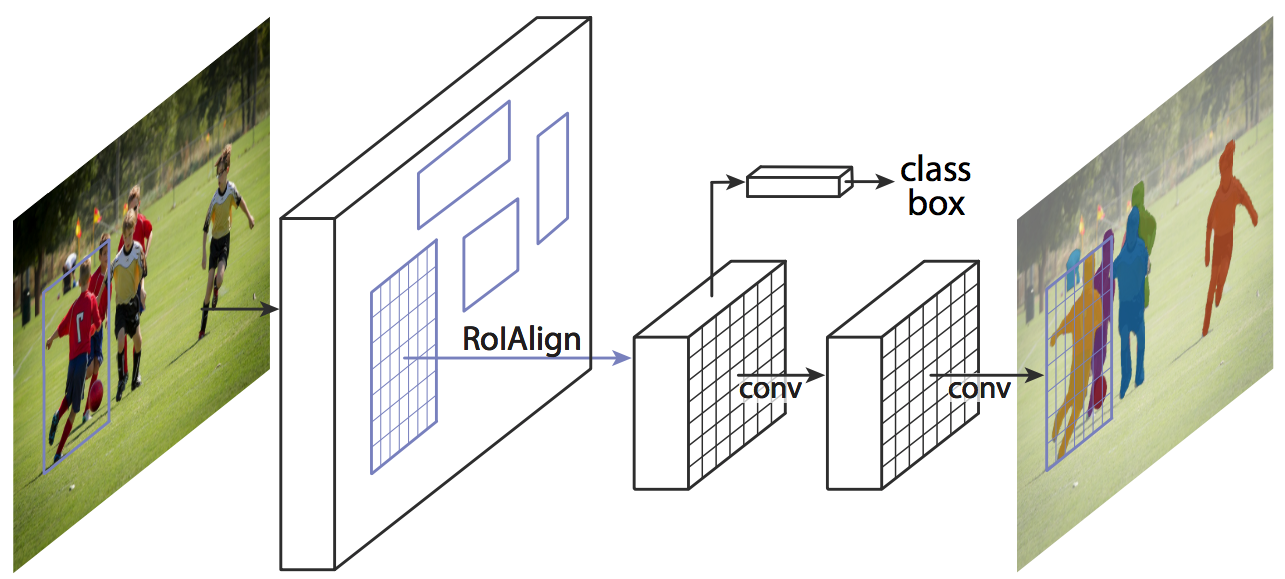
\includegraphics[scale=.2]{image/maskrcnn}
    \end{center}
    \caption{Mask RCNN}
    \end{figure}
\end{center}

Dựa trên kiến trúc của Faster RCNN, Mask RCNN đã thêm một nhánh để thực hiện phân đoạn, độc lập với việc phát hiện, bao đóng vật thể. Để có thể phân loại từng pixel trong ảnh một cách chính xác, Lớp ROIAlign sẽ thay thế cho ROIPool để ko đánh mất thông tin trong featuer map khi trích xuất nó về một feature map nhỏ hơn. Đây cũng là một trong những điểm nhấn, cải tiến quan trọng của Mask RCNN để đạt được những kết quả tốt hơn trong việc phân đoạn. Từ những feature map lấy được, Mask RCNN áp dụng Fully Convolution Network (FCN) để thực hiện việc phân đoạn. 




